\documentclass{article}

\usepackage{graphicx}
\usepackage[left=2cm,top=1cm,right=3cm]{geometry}

\begin{document}
\setlength{\parindent}{0pt}
\setlength{\parskip}{.5ex plus 0.5ex minus 0.2ex}


% \setlength{\parskip}{8pt}
% \setlength{\parsep}{8pt}


\title{ drawnTogether -- a collaborative approach to virtual graffiti }

\author{ Jeremy Kelley, Kyumin Lee, \& Xiheng Zhang }

\date{\today}

\maketitle

\section{ Abstract }

In this work, we propose and implement a new application enabling ubiquitous
creation of virtual graffiti, intended to support location awareness and
interaction amongst mobile peoples despite their lack of temporal co-location.
In particular, we developed a mobile application using the GPS and compass
within the iPhone 3G S to allow participants to create sketches attached to
real world geographic locations and others to view them and contribute at a
later time.  We intend to show user interaction rates among participants
increasing when they can contribute to something permanently, even in the
digital sense.

\section{ Contribution and Benefits Statement }

\begin{quote}
Describes a system enabling ubiquitous creation of virtual graffiti, intended
to support location awareness and interaction amongst mobile people despite
their lack of temporal co-location.
\end{quote}

\section{ Prior Work Analysis }

Zurita et al. \cite{sketching:zurita} presents MCSketcher, a mobile
collaborative sketching system, using handheld devices in an ad-hoc network.
People can draw sketches with collaborators in the same page in the system.
They can take a picture and use it in the background of the drawing. The system
supports gesture recognition for basic navigation gestures, and selecting and
resizing items. Collaborative work is only available in an ad-hoc network. In
other words, friends or collaborator can only work together in close distance.
Our application connects to a server to store what users draw and to retrieve
what they drew in the past using cellular networks. One can collaborate with
not only friends, but also any people.

Kim and Dey \cite{augmented_reality:kim} presents displaying augmented reality
based car navigation information on windshield. Augmented reality helps elder
people can concentrate to drive a car and easily follow directions from a
navigation system. Augmented reality is one of ways to display various
information in a view. Likewise, overlapping sketches can help for users to
know what has happened in a certain location, even though augmented reality is
not exactly applied to our application. In addition, our application provides
users with some filters such as name of a drawer, time and so on, so that they
can select what they want to view.

Bast\'{e}a-Forte and Yen \cite{brainstorming:marcello} presents a collaborative
sketching tool. Each user has a Tablet PC to draw some sketches and to view
shared sketches. Each userÕs drawling is synchronized, so that users can view
the same drawling. The collaborative sketching tool helps each userÕs
contribution is equalized although it reduces total number of sketches. Our
application enables users to collaborate drawing no matter what their
relationship is.

The authors in \cite{context:weis} are trying to combine various context-aware
applications. They want to retrieve data from different sources and services,
thus design a general purpose client software that can be used to access a
variety of context-aware services. In their paper, they proposed an
architecture of their system model. They use messenger protocols. If a service
has new information, it sends a short notification message via the servers to
the client. The client can then decide whether it wants to retrieve the full
data. Therefore, the client can directly connect to the service. A discovery
service is used to find services which are relevant for a client in its current
context. It uses the messenger protocol to inform the client software about new
services. In our project, we will find sketches relevant for a client based on
its current context information - both GPS data and twitter friends.

 The authors in \cite{ink:lindell} tested a few hardware and software
technologies in real-time collaborative system, basically raised two
fundamental principles - collaboration and persistence. The two principles
refer to the ability to communicate ideas with other interested parties in
real-time and the ability to store the results of those interactions for
long-term reference, respectively. The softwares include NetMeeting, OneNote,
DyKnow. Their work is mainly to help students share class materiel and
simultaneously edit presentation text or  sketch.

\section{ Revised Proposal }

\begin{figure}
\centering
\includegraphics[width=.45\textwidth]{arch.pdf}
\caption{A simplified diagram showing client communications}
\label{fig:arch}
\end{figure}

\begin{figure}
\centering
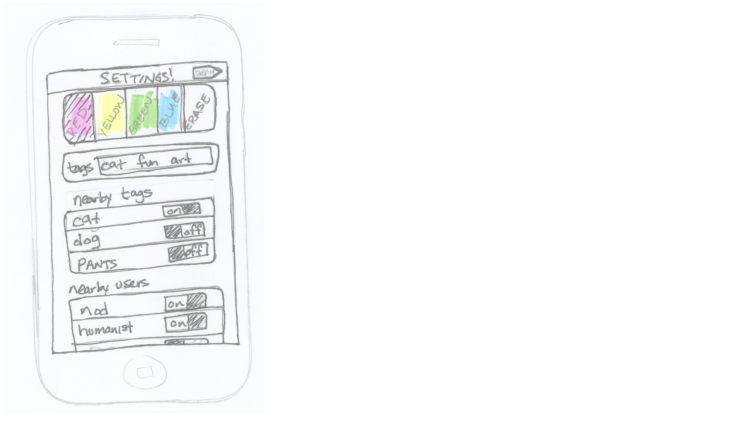
\includegraphics[width=.35\textwidth]{settings.pdf}
\caption{A mockup of the proposed settings interface}
\label{fig:settings}
\end{figure}


\begin{figure}
\centering
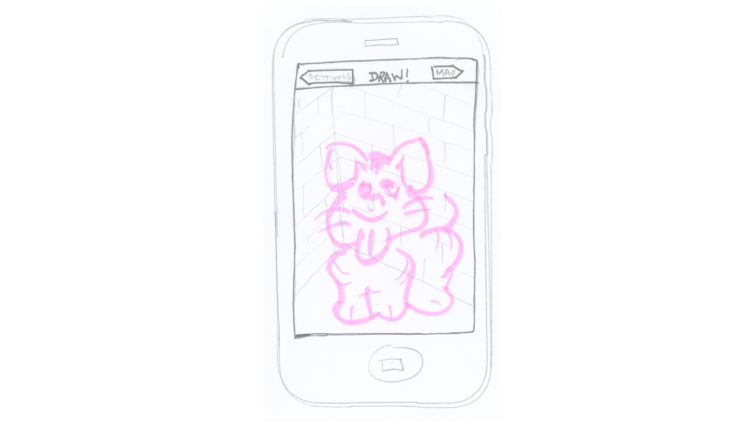
\includegraphics[width=.35\textwidth]{draw.pdf}
\caption{A mockup of the proposed drawing interface}
\label{fig:settings}
\end{figure}

\begin{figure}
\centering
\includegraphics[width=.35\textwidth]{map.pdf}
\caption{A mockup of the proposed map interface}
\label{fig:map}
\end{figure}

We are going to develop a collaborative artistic application for the iPhone 3GS. This application allows users raw sketches on their iPhone and upload the sketch as well as their global position and orientation at that moment, to a server. The sketch can be anything the user wants to draw. It can be the view he/she is seeing, or the idea he/she is thinking about, or his mood and his feeling. The purpose of this application is to help users collaborate and communicate better with others in the same network, or let actors be more aware of what happened around based on context information and more involved in social activities. The context information contains both temporal and spatial information. Each sketch will be timestamped at the point it is uploaded to the server.

The spatial data has:
\begin{enumerate}
\item the current position the user locates, indicated by x (latitude), y (longitude) and z (altitude) available via GPS in the devi
ce.
\item the current orientation the user faces available via the magnetic compass within the device.
\end{enumerate}
The orientation is important because view would be affected given different orientation.

Just like common social networks, users have his/her own networks in our system. i.e., one may only interested in his/her friends' s
ketches or sketches of people who have a same interest with him/her. Also, users can choose his/her sketch to be public, private or 
only share with friends. Due to the huge amount of data in server, users need the ability to filter contributions based on his/her p
references. This refine process will be discussed in our next step of work.


The specific activities users will conduct using our system include:
\begin{enumerate}
\item Hold iphone in hand, stay at any location GPS can track.
\item On the iphone screen, make some sketch as seen in Figure \ref{fig:draw}
\item For sketch, users can paint in a limited number of colors and have that
	creation tagged as seen in Figure \ref{fig:settings}
\item As the sketch is created, it will be uploaded to the server at small
	increments (every $n$ seconds)
\item Users can retrieve entries based on a simple query interface. Thus
	conditions involve: social relations, tag, time, and present location.
\item Users can view which sketches are near them via a map interface, as seen
	in Figure \ref{fig:map}
\end{enumerate}

Here is an initial description of the components we will need to prototype for
the system (hardware and software)

\begin{enumerate}
\item Client interface
        \begin{itemize}
        \item iPhone 3GS
        \item  Sketch application
        \end{itemize}

\item Web service
        \begin{itemize}
        \item Operating system: Linux
        \item Web server: Lighttpd
        \item Web application: custom service build using Django framework
        \item Database: MySQL
        \item Code management tool during development: git
        \end{itemize}
\end{enumerate}


\section{ Evaluation Plan }

All people who own an iphone may be interested in this system, especially young
people in university. If interviews and tests need to be conducted during the
course of the project, we prefer do a small group of field study. We first
introduce our system and make them aware how useful and funny our system is.
After users have much experience with the application, we will get their
feedback about this system based on interviews. We may input some random
sketches into our server repository before users are able to view submitted
drawings.

\subsection{Hypotheses}

The sketch application on iphone 3GS should be manipulated conveniently and
effectively. On the screen of iphone 3GS, users can make sketch freely with
four colors. The most significant part of this application is that
collaboration among  users should happen in real time, even with large number
of people drawing for the same object at the same time.

\subsection{Paper Mockup Evaluation}

Before we write the application, we will conduct an interview with 5-10 people
for the mock interactive interface on paper. We will observe what they will
draw on the paper. Of course, the available area on the paper is the same size
as the screen of iphone 3GS. T his part will be done before Nov. 24.

\subsection{Field Study}

After the first version of our application is done (after Dec.1 and before Dec.
5), we will perform ``hands on interviews'' with 5-10 people who have iphone
3GS.  Basically, we will obverse how people are using it and ask them their
opinions about our system.

\subsubsection{Observe users}

We will help users to install the application, but when the installation is
finished, we will not teach them how to use the application, just observe how
users will manipulate in their iphone 3GS screen in each step. During this
process, of course, users will ask questions about what would happen when
touching the interactive screen or in order to show what the user want the
screen to be, what kind of operation should be done? Based on those questions,
we will know what part should be revised in the application. Also, we will see
if the sketch will be updated automatically in real-time among other users'
iphone screen.

\subsubsection{Interview}

After users finish playing with our application, we will ask some questions as
the part of interview.  Here is an initial list of structured-interview
questions:
\begin{itemize}
\item Is this idea interesting? Are you having fun with the new iphone 3GS application?
\item Are the sketch setting options enough for you to draw? If not, what else should be considered?
\item How you like the user interface? Any improvement needed?
\item If you are the designer, what other affordances do you like to add into our application?
\item Will you recommend this application to your friends and play with them together?
\item Is there any problem for this application? Any suggested solutions?
\end{itemize}




\section{Development Plan}

The scope of this project and the tight deadlines means that team communication
and productivity is of the utmost importance.

\subsection{ Application Environment and Development Tools }

\subsubsection{ Mobile Client }

Since the prototype is intended for the iPhone OS, there are few options for
development environments.  The path of least resistance (and greatest
productivity) is for the application to be written in Objective C, and built
using Apple's iPhone SDK toolchain integrated into the Xcode IDE.  It is
possible to develop iPhone applications outside of Xcode, using other text
editors and foregoing the builtin debugging integration that Xcode offers, but
to compile and link, one is still required to use the provided tools by Apple.
For this reason, our team will focus on the Xcode environment and the full
stack that it has to offer.  In particular, we will be using the following:

\begin{itemize}
\item development workstations will run OSX
\item Xcode
\item iPhone 3G S
\item iPhone Simulator
\end{itemize}

\subsubsection{ Web Service }

In order for the applications on the client devices to share content, a
centralized web service is required.  There are many options within this realm,
however, for ease of development since time is short on this prototype, this
web service will be built using the following:

\begin{itemize}
\item Python scripting language
\item Django Web Framework
\item Lighttpd HTTP Server
\item MySQL Database
\item JSON for data transport
\end{itemize}

This stack of tools has been widely utilized in numerous installations and in
particular, the Python language has proven itself to be quite powerful, yet
easy to learn.

\subsubsection{ Version Control \& Source Code Management }

In order to facilitate sharing our work, we have created a repository at
GitHub\footnote{http://github.com}.  This allows us to use Git, a distributed
version control system, for all of our created content.  Our source code,
scripts, and even our papers (written in \LaTeX) will be stored in this shared
repository.  This allows us, as a distributed team working in disparate
locations, to share all content and stay up-to-date with others contributions.

Git also provides issue tracking that we have begun using in an effort to track
progress and discussion on multiple concurrent items.

\subsection{ Development Milestones  }

\begin{itemize}
\item 17 Nov -- Storyboards and Lo-fi Prototypes
\item 19 Nov -- Webservice completed and API locked for data transfer
\item 23 Nov -- pre-Alpha ``Sketchable'' interface working on Sim with fabricated geo data
\item 24 Nov -- Initial User Feedback incorporated into final designs
\item 26 Nov -- Early ``Alpha'' version of the mobile client ready
\item 1 Dec -- Prototype due

\end{itemize}

\subsection{ Application Architecture }

The heart of the mobile application will be the integration of a live video
feed from the device's camera overlaid by user contributed sketches for the
current location of the device.  The application will rely on Apple's
CoreLocation service to provide the location and orientation information in
order to retrieve user content from the web service.  We will run an NSTimer
that will create NSInvocationOperations at regular intervals to submit any user
created content in the background during viewing and to retrieve any new
content for the user's current geographic area.

We intend to incorporate a simple user identity component using Twitter.  This
will allow us to attach a user to a sketch without having to manage the
identity infrastructure.  By having identity information attached to each
contribution, we will also have the ability to allow users to filter based upon
the user.

There will be a tagging component, although it will be limited in this initial
prototype.  The user will be able to create a set of tags that will be applied
to sketches created after tag assignment.

Finally, a map view will be provided which will indicate to the user sketches
near to them, to allow for ``sketch tours'' or other artistic discoveries.

\section{Scenarios}
We can apply our application to various scenarios. In this section, we show two
of them.

\subsection{Scenario 1: collaborative drawing}

Alice and Bob are students at Texas A\&M University and are friends. Alice
wanted to draw the MSC building before it is remodeled, so she went near to the
building and sketched it using our application. She did not finish the drawing
because of a class. While she is going to a classroom, she sends a SMS message
to Bob. The message is ``Could you finish the sketch for the MSC building in
location X?'' Fortunately, he is passing in front of the building and starts to
add some sketch into the figure, which Alice drew. Sometimes later, he finishes
to draw the building and sends a SMS message to her. The message is ``I'm
done!'' After the class is finished, she goes to the location in which she drew
the building. She can view what they drew and is satisfied about what they did.

\subsection{scenario 2: recalling a old building}

Now the MSC building is under construction. George is a new student at TAMU. He
hears about the old MSC building from senior friends, but he does not know what
exactly it looked like and what happened near to the MSC building in the past.
His senior friend tells him to use our application to view the scenes because
some students drew the building and scenes near the building in the past,
leaving some comments. He can view stored scenes and filter them by a drawer,
time and so on. Even though the building is under construction, new students
including George can recall it.




%%%%%%%%%%%%%%%%%%%
\bibliographystyle{plain}
\bibliography{../bibli} 
\end{document}
